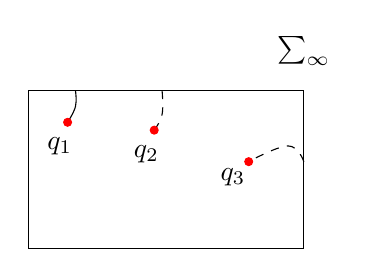
\begin{tikzpicture}

\draw  (-2,3) rectangle (1.5,1);
\node at (1.5,3.5) {$\sum_\infty$};
\draw  plot[smooth, tension=.7] coordinates {(-1.4,3) (-1.4,2.8) (-1.5,2.6)};
\draw [fill, red] (-1.5,2.6) circle (0.05);
\node at (-1.6,2.3) {$q_1$};
\draw [dashed] plot[smooth, tension=.7] coordinates {(-0.3,3) (-0.3,2.7) (-0.4,2.5)};
\draw  [fill, red] (-0.4,2.5) circle (0.05);
\node at (-0.5,2.2) {$q_2$};
\draw  [dashed]plot[smooth, tension=.7] coordinates {(1.5,2.1) (1.3,2.3) (0.8,2.1)};
\draw   [fill, red](0.8,2.1) circle (0.05);
\node at (0.6,1.9) {$q_3$};
\end{tikzpicture}